\documentclass[11pt,a4paper,titlepage]{article}
\usepackage[a4paper]{geometry}
\usepackage[utf8]{inputenc}
\usepackage{xeCJK}
\usepackage{parskip}
\usepackage{indentfirst}

\setmainfont{Helvetica}
\setCJKmainfont{PingFang SC}

\usepackage{lipsum}
\usepackage[english]{babel}
\usepackage{url}
\usepackage{amsmath, amssymb, amsfonts, amsthm, fouriernc, mathtools}
% mathtools for: Aboxed (put box on last equation in align envirenment)
\usepackage{microtype} %improves the spacing between words and letters

%--------------------------------------------------------------------------
%% Code
%--------------------------------------------------------------------------
\usepackage{graphicx}
\usepackage{subcaption}
\graphicspath{{figures/}}

%--------------------------------------------------------------------------
%% Code
%--------------------------------------------------------------------------
\usepackage{listings}
\usepackage{color,xcolor}
\definecolor{mygreen}{rgb}{0,0.6,0}
\definecolor{mygray}{rgb}{0.5,0.5,0.5}
\definecolor{mymauve}{rgb}{0.58,0,0.82}
\newfontfamily\monaco{Monaco}
\lstset{
backgroundcolor=\color{white},   % choose the background color
basicstyle=\tiny\monaco, % size of fonts used for the code或改成\small\monaco稍大
numbers=left,                        % 设置行号
numberstyle=\tiny\monaco,            % 设置行号字体大小
columns=fullflexible,
breaklines=true,                 % automatic line breaking only at whitespace
captionpos=b,                    % sets the caption-position to bottom
tabsize=2,
commentstyle=\color{mygreen},    % 设置注释颜色
escapeinside={\%*}{*)},          % if you want to add LaTeX within your code
keywordstyle=\color{blue},       % 设置keyword颜色
stringstyle=\color{mymauve}\monaco,     % string literal style
frame=single,                        % 设置有边框
rulesepcolor=\color{red!20!green!20!blue!20},
% identifierstyle=\color{red},
language=Octave,
}

%--------------------------------------------------------------------------
%% PREPARE TITLE
%--------------------------------------------------------------------------
\newcommand{\HRule}[1]{\rule{\linewidth}{#1}}
\title{ 
  \HRule{0.5pt} \\
  基于遗传算法的多阈值图像分割 \\
  \HRule{2pt} \\ [0.5cm]}
  
\author{\\[3cm]
  安雅萌\\[0.1cm]
  181270005\\[0.1cm]
  }
\date{网络空间安全学院}
%--------------------------------------------------------------------------


\begin{document}
\maketitle
\setmainfont{Helvetica}
\setlength{\parindent}{2em}

\section{引言}

图像分割是区分图像中物体和背景的过程,由于图像具有不同形式的直方图,如何确定合适的阈值对图像进行分割是该算法的关键。本文采用了遗传算法来寻找图像分割的阈值,算法的目标是最大化物体和背景之间的类间方差,并最小化物体像素之间和背景像素之间的类内方差\cite{gonzalez2002digital}。

图像阈值通常使用一个阈值将灰度图像退化为二值图像,低于该阈值的像素将被视为背景,高于该阈值的像素将被认为是物体。对于一个彩色图像,首先需要将其转换为灰度图像,再进行阈值分割处理。阈值分割方法包括单阈值分割和多阈值分割。其中,多阈值分割通过使用若干阈值来区分图像中多个不同的物体\cite{banimelhem2011multi},不同阈值有$256\times255\times...(256-t-1)$种可能。如果采用暴力求解的方式可以求得最优解,但是计算量太大了,而采用遗传算法可以高效地求得近似最优解。

遗传算法是计算数学中用于解决最优问题的搜索算法,通常包括种群初始化、适应性评估、繁殖和终止四个阶段\cite{mitchell1998introduction}。其中繁殖包括选择、交叉、突变和接受解四个步骤。在选择步骤中,通过选择当前种群中适应性最好的个体来繁殖产生新的个体,本文为了实现方便每次选择时选出新一代的最优解。

\section{实现算法}

本方法所使用的染色体为一个长度为 $log(256)\times n$ 的字符串,其中 $n$ 为阈值个数,每 组的$log(256)$个字符表示一个阈值。首先,找到图像的直方图,直方图信息将用于适应性评估。然后随机初始化若干个染色体。之后迭代一定的次数,最终选出最优见。主要代码如下所示,实验环境为 GNU Octave。

\subsection{初始化}
为了保证种群的大小在迭代时保持不变,需要使选择、交叉和突变的比率满足 $n\_selection + n\_crossovers + n\_mutation = 1$。主要参数如下:
\begin{itemize}
  \item n\_population:种群规模;包含不同的解
  \item n\_iterations:迭代次数;迭代完成后算法终止
  \item n\_thresholds:所需阈值的数量;n个阈值能够将图像分割成n+1块
\end{itemize}

\begin{lstlisting}[
  numbers=left,
  numberstyle=\tiny\monaco,
  basicstyle=\scriptsize\monaco]
pkg load image

% Default variables
n_population =  20;
n_iterations =  50;
n_bins       = 256;
n_thresholds =   5;

% Ratios of all GA operations
p_selection = 0.1;
p_crossover = 0.8;
p_mutation  = 0.1;
assert(sum([p_selection, p_crossover, p_mutation]) == 1, 'Total sum of proportions have to be 1!');

% Read image
image = imread("images/img.png");

% Convert image to gray levels
if (size(image, 3) == 3)
    image_gray = rgb2gray(image);
else
    image_gray = image;
endif

% Initialization
population = initialization(n_population, n_bins, n_thresholds);

for i = 1:n_iterations
    new_population = [];

    % Evaluation of fitness
    ranking = fitness(image, population, n_thresholds);

    %% Reproduction
    % Selection
    % TODO create more strategies (like roulette wheel)
    new_population = first_best(ranking, population, p_selection, new_population);

    % Crossover
    new_population = crossover(population, p_crossover, new_population);

    % Mutation
    new_population = mutation(population, p_mutation, new_population);

    population = new_population;
endfor

% Accepting the solution
accept_solution(image_gray, population, n_thresholds);
\end{lstlisting}

\subsection{适应性评估}

适应性通过物体和背景的类间方差及类内方差来确定,由于大津已经证明了最小化类内方差和最大化类间方差是相同的\cite{otsu1979threshold},本方法选择计算类内方差,总和最低的方案即为最优解。

\begin{lstlisting}[
  numbers=left,
  numberstyle=\tiny\monaco,
  basicstyle=\scriptsize\monaco]
function ranking = fitness(image, population, n_thresholds)

  ranking = [];

  % Convert thresholds to decimal representation
  thresholds =  convert_thresholds(population, n_thresholds);

  % Vectorize image
  image_vec = image(:);

  % Computes fitness ranking for all thresholds in population
  for i = 1:size(thresholds, 1)
      ranking = [ranking; fitness_one(image_vec, thresholds(i,:))];
  endfor

endfunction
\end{lstlisting}

\begin{lstlisting}[
  numbers=left,
  numberstyle=\tiny\monaco,
  basicstyle=\scriptsize\monaco]
function ranking = fitness_one(image_vec, thresholds_vec)

  ranking = 1;
  inter_var = 0;
  intra_var = 0;

  % Sort thresholds
  thresholds_vec = sort(thresholds_vec);

  end_i = size(thresholds_vec, 2) + 1;
  for i = 1:end_i
      if ((i == 1 && end_i == 2) || i == 1)
      % One threshold or the first threshold
          left = 0;
          right = thresholds_vec(i);
      elseif (i == end_i)
      % The last threshold
          left = thresholds_vec(i-1);
          right = max(image_vec);
      else
      % More thresholds
          left = thresholds_vec(i-1);
          right = thresholds_vec(i);
      endif

          % <0; x) <x; y) <y; max(image_vec))
          left_mask = image_vec >= left;
          right_mask = image_vec < right;
          mask = left_mask .* right_mask;
          object = image_vec(find(mask));

      % TODO better way to relate all variances within objects?
      if (length(object) == 0)
          variance = 1;
      else
          variance = var(object);
      endif

      ranking = ranking + variance;
  endfor

endfunction
\end{lstlisting}

\subsection{选择}

目前的解决方案是只选择新一代最优解,数量取决于比率 n\_selection。

\begin{lstlisting}[
  numbers=left,
  numberstyle=\tiny\monaco,
  basicstyle=\scriptsize\monaco]
function new_population = first_best(ranking, population, p_selection, new_population)

  population_size = size(population, 1);
  [best, best_i] = sort(ranking);

  for i = 1:round(p_selection*population_size)
      new_population = [new_population; population(best_i(i), :)];
  endfor

endfunction
\end{lstlisting}

\subsection{交叉}

交叉是指两条染色体在配对时互换部分染色体,交叉的染色体数量取决于比率 n\_crossover。本方法采用单点交叉的方式,交叉点随机生成,均匀分布。

\begin{lstlisting}[
  numbers=left,
  numberstyle=\tiny\monaco,
  basicstyle=\scriptsize\monaco]
function new_population = crossover(population, p_crossover, new_population)

  population_size = size(population, 1);

  % Random permutation of genomes order 
  parent_first = randperm(population_size);
  parent_second = randperm(population_size);

  % Number of couples used for crossover
  n_crossovers = round(p_crossover*population_size)/2;

  for i = 1:n_crossovers
      % Crossovers parents
      [desc_first desc_second] = crossover_one(population(parent_first(i),  :), population(parent_second(i), :));

      % Add crossover descendants
      new_population = [new_population; desc_first; desc_second];
  endfor

endfunction
\end{lstlisting}

\begin{lstlisting}[
  numbers=left,
  numberstyle=\tiny\monaco,
  basicstyle=\scriptsize\monaco]
function [desc_first desc_second] = crossover_one(parent_first, parent_second)

  parent_size = size(parent_first, 2);

  % Randomly generated number between 1 and the length of parent's genome.
  point = round(unifrnd(1, parent_size-1));

  % Crossover
  desc_first  = [parent_first(1:point)   parent_second(point+1:parent_size)];
  desc_second = [parent_second(1:point)  parent_first(point+1:parent_size)];

endfunction
\end{lstlisting}

\subsection{突变}

染色体的序列是随机排列的,并且排在首位的更可能被选择。突变的染色体数量取决于比率 n\_mutation。目前的解决方案是只允许突变一个染色体基因。

\begin{lstlisting}[
  numbers=left,
  numberstyle=\tiny\monaco,
  basicstyle=\scriptsize\monaco]
function new_population = mutation(population, p_mutation, new_population)

  population_size = size(population, 1);

  % Random permutation of genomes order 
  mutation_order = randperm(population_size);

  for i = 1:round(p_mutation*population_size);
      new_population = [new_population; mutate_one(population(mutation_order(i), :))];
  endfor

endfunction
\end{lstlisting}

\begin{lstlisting}[
  numbers=left,
  numberstyle=\tiny\monaco,
  basicstyle=\scriptsize\monaco]
function new_chromosome = mutate_one(chromosome)

  new_chromosome = chromosome;

  chromosome_size = size(chromosome, 2);
  gene = round(unifrnd(1, chromosome_size));

  % Mutate one gene
  if (chromosome(gene) == 1)
      new_chromosome(gene) = 0;
  else
      new_chromosome(gene) = 1;
  endif

endfunction
\end{lstlisting}

\section{实验效果}

\subsection{二值分割}

\begin{figure}[!htb]
  \begin{subfigure}{\linewidth}
  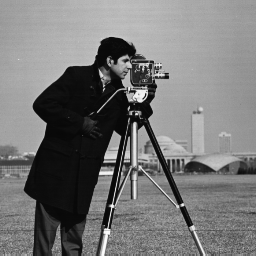
\includegraphics[width=.3\linewidth]{cameraman.png}\hfill
  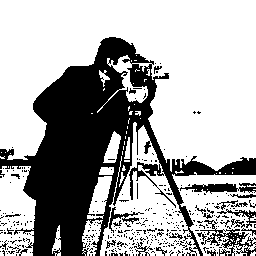
\includegraphics[width=.3\linewidth]{ga-cameraman.png}\hfill
  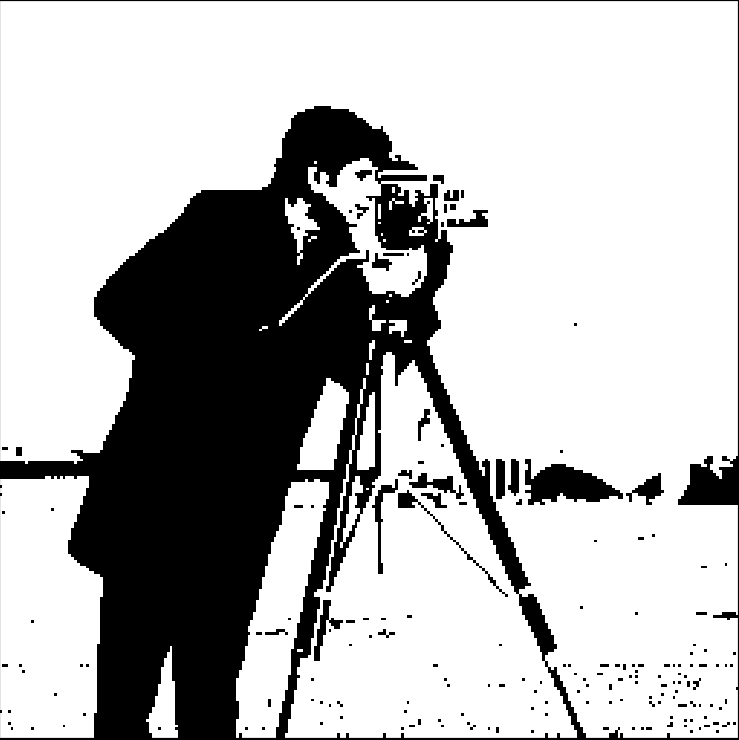
\includegraphics[width=.3\linewidth]{otsu-cameraman.png}
  \end{subfigure}\par\medskip
  \caption{二值分割效果比较\\
  左至右:原始图片,本文算法(种群大小为20,迭代30次),Otsu}
\end{figure}

\subsection{多阈值分割}

本文使用工具\cite{benchmark}对20张合成的纹理图进行测试,种群数为20,迭代次数为50。以下包括两组测试示例,每组图片从左至右依次为原始图片、理论分割结果、遗传算法分割结果。从图中可以看出分割的结果并不是很好,总体准确率有2.17\%。

\begin{figure}[!htb]
  \begin{subfigure}{\linewidth}
  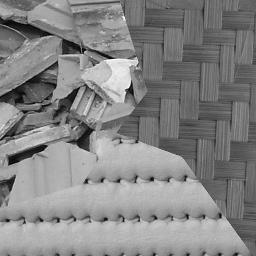
\includegraphics[width=.3\linewidth]{mosaic11.png}\hfill
  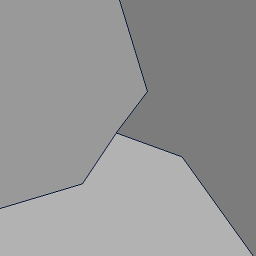
\includegraphics[width=.3\linewidth]{mosaic12.png}\hfill
  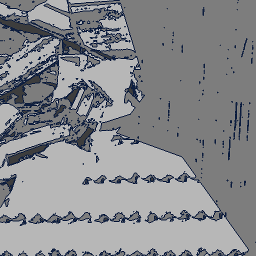
\includegraphics[width=.3\linewidth]{mosaic13.png}
  \end{subfigure}\par\medskip
  \caption{多阈值分割测试1\\
  2个阈值,3块}
\end{figure}

\begin{figure}[!htb]
  \begin{subfigure}{\linewidth}
  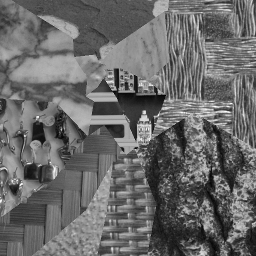
\includegraphics[width=.3\linewidth]{mosaic21.png}\hfill
  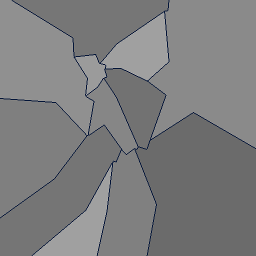
\includegraphics[width=.3\linewidth]{mosaic22.png}\hfill
  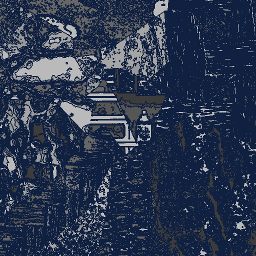
\includegraphics[width=.3\linewidth]{mosaic23.png}
  \end{subfigure}\par\medskip
  \caption{多阈值分割测试2\\
  11个阈值,12块}
\end{figure}

\section{结论}
遗传算法能够找到多阈值分割的近似最优解,但对于二值分割效果不如Otsu算法。本方法的主要缺点在于倾向于分割边缘这样的小区域,但这些区域都是无关紧要的细节,不应考虑在内。

本方法可以通过采用多点交叉和轮盘赌选择法来进行改进,从而避免染色体在几代之后差异减小失去多样性的问题。

%--------------------------------------------------------------------------
%% Reference
%--------------------------------------------------------------------------
\setmainfont{Times-Roman}
\bibliographystyle{unsrt}

\bibliography{article.bib}

\end{document}